\documentclass[a4paper]{article}
\addtolength{\hoffset}
{-2.25cm}
\addtolength{\textwidth}
{5cm}
\addtolength{\voffset}
{-3.25cm}
\addtolength{\textheight}
{5.5cm}
\setlength{\parskip}{0pt}
\setlength{\parindent}{0in}

\usepackage[utf8]{inputenc}
\usepackage{microtype}
\usepackage[english]{babel}
\usepackage{fancyhdr}
\usepackage{advdate}
\usepackage{enumitem}
\usepackage{amsmath, amssymb}
\usepackage{graphicx}
\usepackage{caption}
\usepackage{subcaption}
\usepackage{float}
\usepackage{titlesec}
\usepackage{wasysym}
\usepackage{url}
\usepackage{hyperref}
\usepackage{tikz, verbatimbox}
\usepackage{fixltx2e}
\usepackage{centernot}
\usepackage{algorithm}
\usepackage{algpseudocode}
\usepackage{listings}
\usetikzlibrary{shapes.geometric, arrows}
\usetikzlibrary{positioning}
\usepackage[table]{xcolor}

\graphicspath{{./static/}}
\tikzset{every picture/.style={line width=0.75pt}} %set default line width to 0.75pt

\newcommand{\LComment}[1]{\State \(\triangleright\) \text{#1}}
\MakeRobust{\Call}
\usepackage{pdfpages}

\begin{document}

\fancyhead[c]{}
\hrule \medskip
\begin{minipage}{0.295\textwidth}
\raggedright
Rishabh Indoria\\
21F3001823
\end{minipage}
\begin{minipage}{0.4\textwidth}
\centering
\LARGE
Software Engineering
\end{minipage}
\begin{minipage}{0.295\textwidth}
\raggedleft
\today \hfill \\
\end{minipage}
\medskip \hrule
\bigskip

\section{Thinking of Software in Terms of Components}
\subsection{Case Study: Amazon System}
\begin{itemize}
    \item Components are a way of breaking the complexity of a task into manageable parts, so that different teams can work on different components of the system and put everything in a timely manner.
    \item Everyone need not the working of a component, just need to know the input and output.
    \item Amazon components: Inventory Management, Payment Gateway, Order Management, Shipping System.
    \item Inventory Management is the act of measuring the amount, location, pricing, mix of products available on Amazon.
    \item Inventory gets updated based on current purchasing and seasonal trends.
    \item Payment Gateway is a service that authorizes electronic payments.
    \item \textbf{Key Takeaway}: Software can be divided into separately addressable components called \textbf{modules} that are integrated to satisfy requirements.
    \item Amazon Pay: A mobile wallet, can link credit or debit card information, can link bank accounts, or you can transfer money online to the mobile wallet. Instead of using your debit or credit card to make purchases you can pay with your smartphone that has this mobile wallet. There are many categories like Recharges, Bill payments, Travel and Insurance, etc.
    \item First Step in create a new software component could be \textbf{study existing components of the system}, \textbf{learn a programming language}, \textbf{look at similar systems to understand features}.
    \item \textbf{Study Existing components of the system}: To understand how the new component will interact with existing components.
    \item We need to first understand what is the problem we want to solve?, and based on an analysis of existing or similar systems we need to come up with an explicit set of goals for our own system or for what our implementation should provide.
    \item \textbf{Requirements}: Goals the implemented system should have, and they should cater to the need of clients.
    \item Client can be an external user or internal users. Could be for employees or customers. Client can also be another software as well.
    \item Think about \textbf{who} is going to use your software, for \textbf{what purpose}, and in \textbf{what way}.
    \item \textbf{Key Takeaway}: Requirement specification is the first step in the software development process, through this we need to ensure that the requirements capture clients needs.
\end{itemize}

\subsection{Different phases of Development}
\begin{itemize}
    \item If we went directly to coding after specifying requirements, then we can face issues during integration where different developers may have different ideas about how the functionality should be implemented, difficulties while adding new features that is if I want to add a new feature then it would help to have a big picture view of the system.
    \item \textbf{Software Design}: Big picture view of the software system, provides a structure to the software system.
    \item When a feature is being implemented, multiple developers work together and write code for the feature, they use tools like GitHub to collaborate and write code and very often coding is done in a distributed manner with developers working in different location and even in different time zones. Hence, it is very important that everyone working on the codebase has a consistent understanding of what the code does. For this reason, all developers write \textbf{documentation} for their code and write precise interface definitions.
    \item \textbf{Interface}: An interface is the description of the actions your functions can do without describing the implementation in detail. The interface shows what requests are accepted and in what format is the corresponding response given.
    \item \textbf{Software Development}: Write code based on the requirements and the design. Usually distributed, and the developers write documentation and precise interface definitions.
    \item \textbf{Testing} is done to ensure that the software behaves according to the requirements, many bugs might still exist in the system. A failure to address bugs can even cause severe catastrophes.
    \item Testing is done at different granularities, examples include unit testing, integration testing, acceptance testing.
    \item Alpha testing done by internal employees and Beta testing done by actual users.
    \item \textbf{Maintenance}: After the feature is rolled out, monitor how users are using the feature. Purpose of doing this is to monitor what users are doing, and how they are using the software, change the code for upgrades/updates, or add features.
    \item \textbf{Overall Process}: Requirements $\rightarrow$ Design $\rightarrow$ Development $\rightarrow$ Testing $\rightarrow$ Maintenance
\end{itemize}

\subsection{Software Development Life Cycle}
\begin{itemize}
    \item \textbf{Software Lifecycle}: Different stages over which a software evolves from the initial customer request to a fully developed software.
    \item \textbf{Waterfall model}: Plan and document perspective. Each phase occurs one after the other.
    \item If we follow all phases sequentially, then the time taken could be very long, and if the client doesn't like it or has some changes we will have to start the process all over again.
    \item \textbf{Drawbacks of Waterfall}: Increase in cost, time if changes are required later on. Clients may not know what they need. Designers may not know which design might be the most feasible/usable by the clients. Can take quite long.
    \item \textbf{Prototype Model}: Build a working prototype before the development of the actual software. Prototype usually not used later.
    \item \textbf{Advantages of prototype}: Exact form of solution and technical issues are unclear, and it is useful to get feedback from customers.
    \item \textbf{Disadvantages of prototype}: Increased development costs, bugs can appear later in the development cycle.
    \item \textbf{Spiral Model}: Incrementally build the software and get feedback, refine. Combines advantages of Waterfall and Prototype model. Each iteration can still take a long time.
\end{itemize}

\subsection{Agile Perspective}
\begin{itemize}
    \item \textbf{Agile Manifesto}: Emphasizes individuals and interactions over process and tools, emphasizes over delivering working software rather than comprehensive documentation, emphasizes on customer collaboration over contract negotiation, emphasizes on responding to change over following a plan.
    \item \textbf{Incremental Development}: Teams work together to deliver the product in small increments.
    \item \textbf{Agile Approaches}: Extreme Programming(XP), Scrum(Product is built in a series of iterations known as sprints which are roughly 1–2 weeks long, this helps break done a project into several small byte sized pieces), Kanban(Software to be built is divided into small work items and these are represented on a kanban board allowing team members to see the state of any piece at any given time).
    \item \textbf{When to use Agile/Plan and Document?}: If the answer is no then Agile else Plan and Document
    \begin{itemize}
        \item Is specification required?
        \item Are customers unavailable?
        \item Is the system to be built large?
        \item Is the system to be built complex?
        \item Will it have a long product lifetime?
        \item Are you using poor software tools?
        \item Is the project team geographically distributed?
        \item Is team part of a documentation-oriented culture?
        \item Does the team have poor programming skills?
        \item Is the system to be built subject to regulation?
    \end{itemize}
    \item \href{https://www.atlassian.com/agile}{What is Agile?}
\end{itemize}


\section{Requirements Gathering and Analysis}
\subsection{Case Study: Amazon Seller Portal}
\begin{itemize}
    \item Our vision of what the software should look like and behave is quite different from what the user has in mind.
    \item We want to make sure that developers understand what customers want, customers come to an agreement about their requirements. If this does not happen we could end up with increased cost and iterations.
    \item Amazon wants to develop a portal for sellers. Products which sellers list on the portal will be available for people to buy on the Seller portal.
    \item \textbf{Primary Users}: Frequent users of the system. Example include Independent sellers, Sales team of consumer companies, Independent authors and publishers.
    \item \textbf{Secondary Users}: Do not directly use the system, use the system through an intermediary. Examples include Sales team managers.
    \item \textbf{Tertiary Users}: Do not use the software at all, affected by the introduction of the software, and Influence the purchase of the software. Examples include logistics, shipping companies, banks, people buying on Amazon.
    \item Requirements can be vague or unclear. Requirements can be inconsistent or contradicting. Requirements can be incomplete.
\end{itemize}

\subsection{Identifying Users and Requirements}
\begin{itemize}
    \item \textbf{Questionnaires}: Series of questions designed to elicit specific information from users. Good for getting answers to specific questions from a large group of people. This should be used in conjunction with other techniques.
    \item \textbf{Interviews}: Asking a set of questions, can be face-to-face, telephonic/online interviews. Can be structured, unstructured, or semi-structured. This helps to get people to explore issues, used early to elicit scenarios.
    \item \textbf{Focus Groups}: Get a group of stakeholders to discuss issues and requirements. Advantages include gaining consensus, highlighting areas of conflict, disagreement.
    \item \textbf{Naturalistic Observations}: Spending time with stakeholders as they go about their day-to-day tasks, observing their work in their natural setting. Shadowing a stakeholder, make notes, ask questions, observe.
    \item \textbf{Documentation}: Procedures and rules for a task, steps involved in an activity, regulations governing a task.
    \begin{table}[H]
        \centering
        \begin{tabular}{|c|c|}
            \hline
            \textbf{Technique} & \textbf{Good for} \\
            \hline
            Questionnaires & Answering specific questions\\
            \hline
            Interviews & Exploring issues\\
            \hline
            Focus Groups & Collecting multiple viewpoints\\
            \hline
            Naturalistic Observations & Understanding context\\
            \hline
            Documentation & Procedures, regulations, standards\\
            \hline
        \end{tabular}
    \end{table}
    \item \textbf{Basic Guidelines}: Focus on identifying stakeholders needs, involve all stakeholder groups, use combination of data gathering techniques. Run a pilot session if possible to ensure your data-gathering session is likely to go as planned.
    \item Data gathering is expensive, time-consuming - have to be pragmatic, make compromises.
    \item \textbf{Functional Requirements}: Captures a functionality required by the users from the system.
    \item \textbf{Non-Functional Requirements}: Essentially specifies how the system should behave. Examples include Reliability, Robustness, Performance, Portability, Security, etc.
    \item \textbf{Reliability}: Te extent to which a program behaves the same way over time in the same operating environment.
    \item \textbf{Robustness}: The extent to which a program can recover from errors or unexpected input.
\end{itemize}

\subsection{Software Requirement Specification}
\begin{itemize}
    \item \textbf{Requirement gathering and analysis}: Done by system analyst, along with other members of the software team. Organize these requirements in \textbf{Software Requirements Specification}(SRS) document.
    \begin{table}[H]
        \centering
        \begin{tabular}{|l|c|}
            \hline
            1. Introduction &  \\
            \hspace{1em}1.1 Purpose & \\
            \hspace{1em}1.2 Scope & \\
            \hspace{1em}1.3 Definitions, acronyms, and abbreviations & \\
            \hspace{1em}1.4 References & \\
            \hspace{1em}1.5 Overview & \\
            2. Overall Description & Broad outline and description of the software system\\
            \hspace{1em}2.1 Product Perspective & \\
            \hspace{1em}2.2 Product Functions & \\
            \hspace{1em}2.3 User Characteristics & \\
            \hspace{1em}2.4 Constrains & \\
            \hspace{1em}2.5 Assumptions and Dependencies & \\
            \hline
            3. Specific Requirements & \\
            \hspace{1em}3.1 External Interface Requirements & \\
            \hspace{2em}3.1.1 User Interfaces & \\
            \hspace{2em}3.1.2 Hardware Interfaces & \\
            \hspace{2em}3.1.3 Software Interface & \\
            \hspace{2em}3.1.4 Communication Interfaces & \\
            \hspace{1em}3.2 System Features & \\
            \hspace{2em}3.2.1 System Feature I & \\
            \hspace{3em}3.2.1.1 Introduction/Purpose of Feature & \\
            \hspace{3em}3.2.1.2 Stimulus/Response Sequence & \\
            \hspace{3em}3.2.1.3 Associated Function Requirements & Functional and Non-Functional Requirements\\
            \hspace{4em}3.2.1.3.1 Functional Requirement I & \\
            \hspace{4em}... & \\
            \hspace{4em}3.2.1.3.n Functional Requirement n & \\
            \hspace{2em}3.2.2 System Feature 2 & \\
            \hspace{2em}... & \\
            \hspace{2em}3.2.m System Feature 2 & \\
            \hspace{1em}3.3 Performance Requirements & \\
            \hspace{1em}3.4 Design Constraints & \\
            \hspace{1em}3.5 Software System Attributes & \\
            \hspace{1em}3.6 Other Requirements & \\
            \hline
        \end{tabular}
        \caption{Standard Structure of SRS document}
        \label{tab:SE-SRS-doc}
    \end{table}
    \item table \textcircled{\raisebox{-0.9pt}{\ref{tab:SE-SRS-doc}}} is a guideline of how an SRS document should look like and is not very rigid.
    \item SRS helps form an agreement between customers and developers. It helps to reduce future reworks. Provides a basis for estimating costs and schedules.
\end{itemize}

\subsection{Behavior Driven Design - User Stories}
\begin{itemize}
    \item Plan and Document perspective requires customers to be clear about their requirements before building the software, but if they are unsure of the requirements then we can follow agile perspective.
    \item \textbf{Behaviour Drive Design}: Asks questions about the behaviour of an application before and during development. Requirements are continuously refined to meet user expectations.
    \item \textbf{User Stories}: Short, Informal, plain language description of what a user wants to do within a software product which is of value of them. Smallest unit of work which can be done in 1 sprint, which is about 1–2 weeks.
    \item Role-feature-benefit pattern/template: As a [type of user], I want [an action], So that [a benefit/value].
    \begin{figure}[H]
        \centering
        \begin{subfigure}[b]{0.45\textwidth}
            \centering
            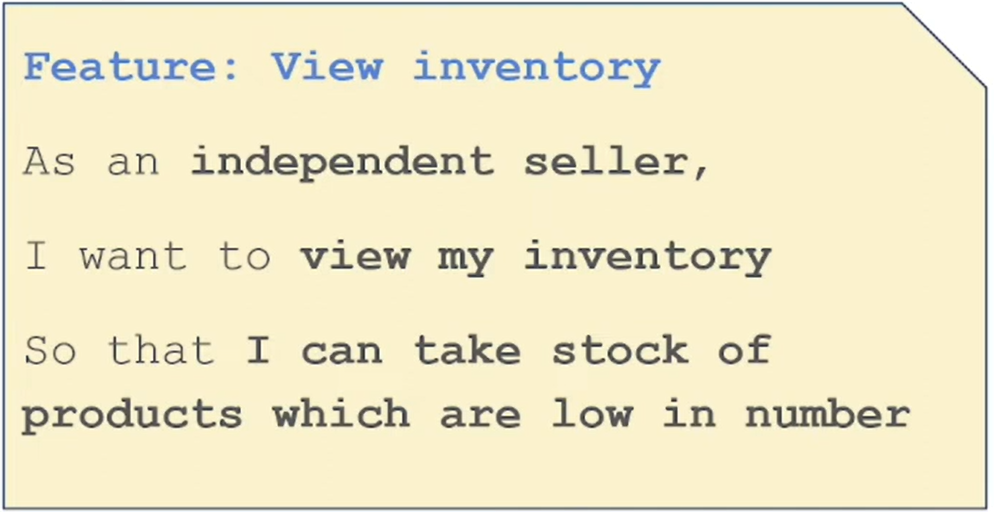
\includegraphics[width=\textwidth]{Degree/static/SE_user_story_1.png}
        \end{subfigure}
        \hfill
        \begin{subfigure}[b]{0.45\textwidth}
            \centering
            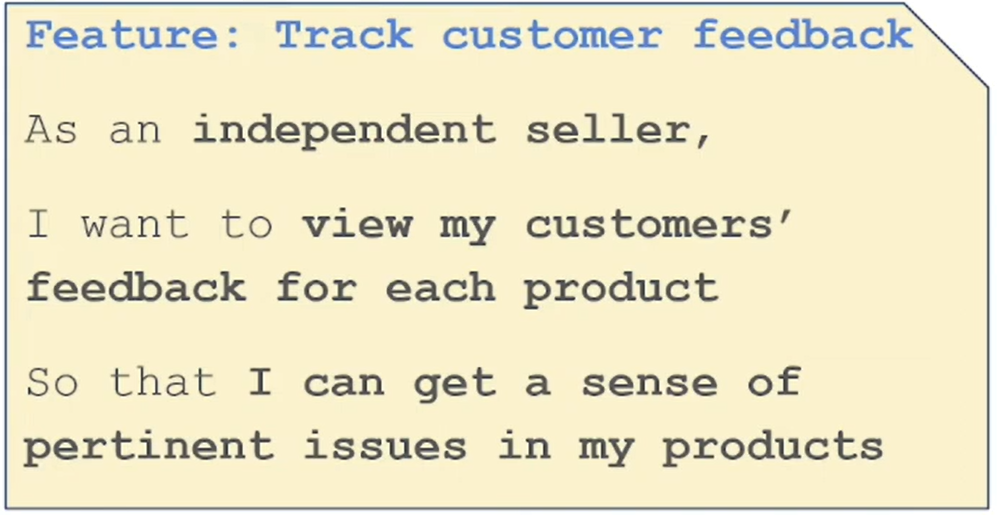
\includegraphics[width=\textwidth]{Degree/static/SE_user_story_2.png}
        \end{subfigure}
        \caption{User Story Examples}
        \label{fig:SE-user-stories}
    \end{figure}
    \item User Stories are lightweight and help plan and prioritize development. Concentrate on behaviour rather than implementation of the application. Conversation between users and the development team.
    \item \textbf{SMART}: Specific(know exactly what to implement), Measurable(known expected results for some inputs), Achievable(Implement the user story in 1-2 weeks), Relevant(Business value to one or more stakeholders), Timeboxed(Stop implementing a feature once time budget expected).
    \item May be difficult to have continuous contact with users. Not able to scale to very large projects, safety critical applications.
    \item \href{https://www.youtube.com/watch?v=KP0U3I-f9-Y}{Brief overview of the difference between requirements and user stories}.
\end{itemize}

\section{Software User Interfaces}
\subsection{Introduction to Interfaces}
\begin{itemize}
    \item Most user stories, require us to create a user interface or a UI that acts as an interaction point between the user and the software.
    \item Activities involved in Interaction Design include identifying needs and requirements, developing alternative design that meet those requirements, Build interactive versions, and Evaluate each of these designs are useful for the user.
    \item \textbf{Usability}: The extent to which a product can be used by specified end users to achieve specified goals with effectiveness, efficiency and satisfaction in a specified context of use.
    \begin{enumerate}
        \item \textbf{Effectiveness}: How good a system is at doing what it is supposed to do.Is the system capable of allowing people to learn well, carry out their work efficiently, access the information they need, buy the goods they want etc.
        \item \textbf{Efficiency}: How does a system support users in carrying out their tasks. Common tasks through minimal number of steps.
        \item \textbf{Safe to use}: Protecting the user from dangerous conditions and undesirable situations. Helping users in any situation to avoid carrying out unwanted actions accidentally.
        \item \textbf{Learnability}: How easy a system is to learn to use. Want to get started right away and carry out tasks without much effort.
        \item \textbf{Memorability}: How easy a system is to remember how to use, once learned.
    \end{enumerate}
    \item \textbf{User Experience Goals}: Want users to experience positive emotions while using the software, More subjective, How users experience a product from their perspective.
    \item \textbf{Prototypes} allow you to quickly test on users, get feedback, iterate, and pivot.
    \item Prototypes answer questions and support designers in choosing between alternatives.
    \item \textbf{Prototyping}: Test out technical feasibility of an idea, clarify some vague requirements, and User testing and evaluation.
    \item \textbf{Storyboard}: A hand drawn comic that features Setting, Sequence, and Satisfaction
    \begin{enumerate}
        \item \textbf{Setting}: People involved, Environment, Task being accomplished
        \item \textbf{Sequence}: What steps are involved? What leads someone to use the app? What task is being illustrated?
        \item \textbf{Satisfaction}: What motivates people to use the system? What does it enable people to accomplish? What need does the system fill?
    \end{enumerate}
    \item \textbf{Benefits of Storyboard}: Emphasizes how interface accomplishes a task. Avoids commitment to a particular user interface. Shared understanding among stakeholders. Some resources \href{https://www.youtube.com/watch?v=JMjozqJS44M}{video-1} and \href{https://www.youtube.com/watch?v=6dre0P4tRTc}{video-2}.
    \item \textbf{Paper Prototypes}: Hand-drawn interface on multiple pieces of paper. 
    \item \textbf{Benefits of Paper Prototypes}: Easier than writing code for user interface. Starts conversation about user interactions. Elements can be changed immediately based on given feedback.
    \item \textbf{Digital Mock-ups}: Using stuff like photoshop, PowerPoint, transform a paper prototype into a digital mockup.
    \begin{figure}[H]
        \centering
        \begin{subfigure}[b]{0.45\textwidth}
            \centering
            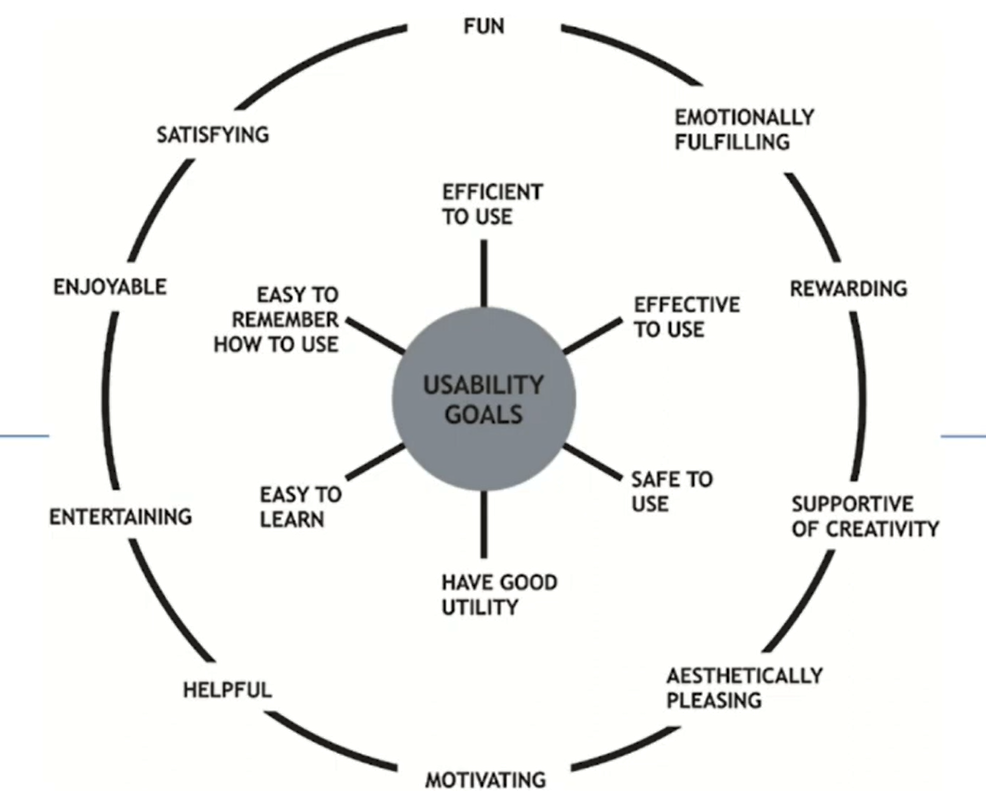
\includegraphics[width=\textwidth]{Degree//static/SE_User_Goals.png}
            \caption{User Goals Summary}
            \label{fig:SE-user-goal-summary}
        \end{subfigure}
        \hfill
        \begin{subfigure}[b]{0.45\textwidth}
            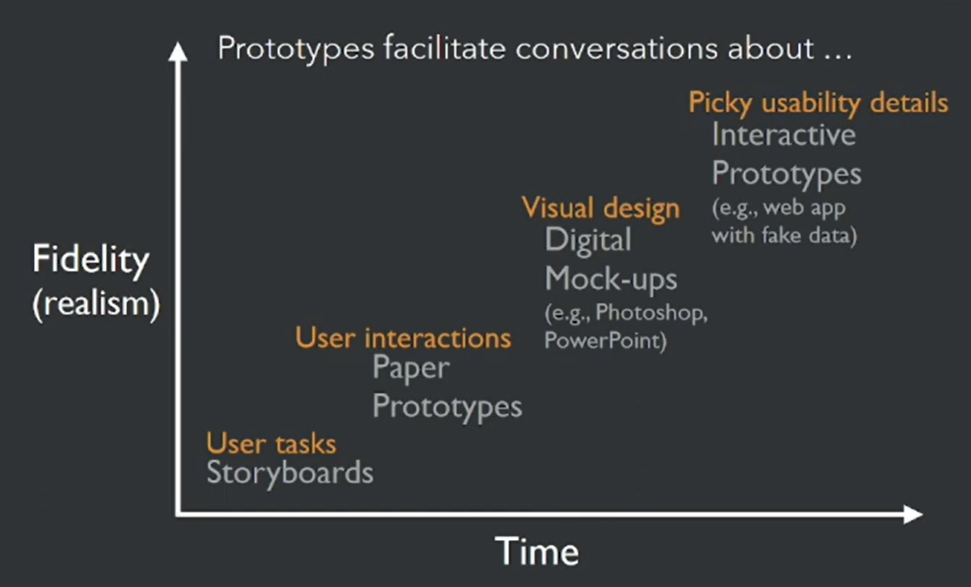
\includegraphics[width=\textwidth]{Degree/static/SE_prototype_summary.png}
            \caption{Prototypes Summary}
            \label{fig:SE-prototype-summary}
        \end{subfigure}
        \caption{Summary of Interfaces}
    \end{figure}
\end{itemize}

\subsection{Evaluation using Design Heuristics}
\begin{itemize}
    \item \textbf{Heuristic Evaluation}: Heuristics are the strategies derived from the previous experiences with similar problems. Rule of thumb/guidelines.
    \item \textbf{Heuristics for Understanding}
    \begin{enumerate}
        \item \textbf{Consistency}: Consistent Layout. Consistent Name.
        \item \textbf{Use Familiar Languages and Metaphors}
        \item \textbf{Clean and Functional Design}
    \end{enumerate}
    \item \textbf{Heuristics for Action}
    \begin{enumerate}
        \item \textbf{Freedom}: Freedom to Undo. Freedom to explore.
        \item \textbf{Flexibility}: Experts as well as new users should be able to carry out tasks efficiently.\\
        \textbf{Personalization}: Tailoring content/functionality for individual users.\\
        \textbf{Customization}: Allow users to make selections about how they want the product to work.
        \item \textbf{Recognition over Recall}: Users find it easier to recognize something they have seen earlier. Interface - buttons, navigation etc. should help the user reach his goal.
    \end{enumerate}
    \item \textbf{Heuristics for Feedback}
    \begin{enumerate}
        \item \textbf{Show Status}: Keep users informed about what is happening, through appropriate feedback within a reasonable amount of time. Provide next steps. Provide warnings in advance.
        \item \textbf{Prevent Errors}: Include helpful constraints. Offer Suggestions.
        \item \textbf{Support Error Recovery}: Make the problem clear. Provide a solution. Provide an alternate.
        \item \textbf{Provide Help}: Ensure help is easy to search. Provide help in context
    \end{enumerate}
    \item Experts evaluate the prototype, i.e., do multiple passes and provide a list of issues that violate design heuristics.
    \begin{figure}[H]
        \centering
        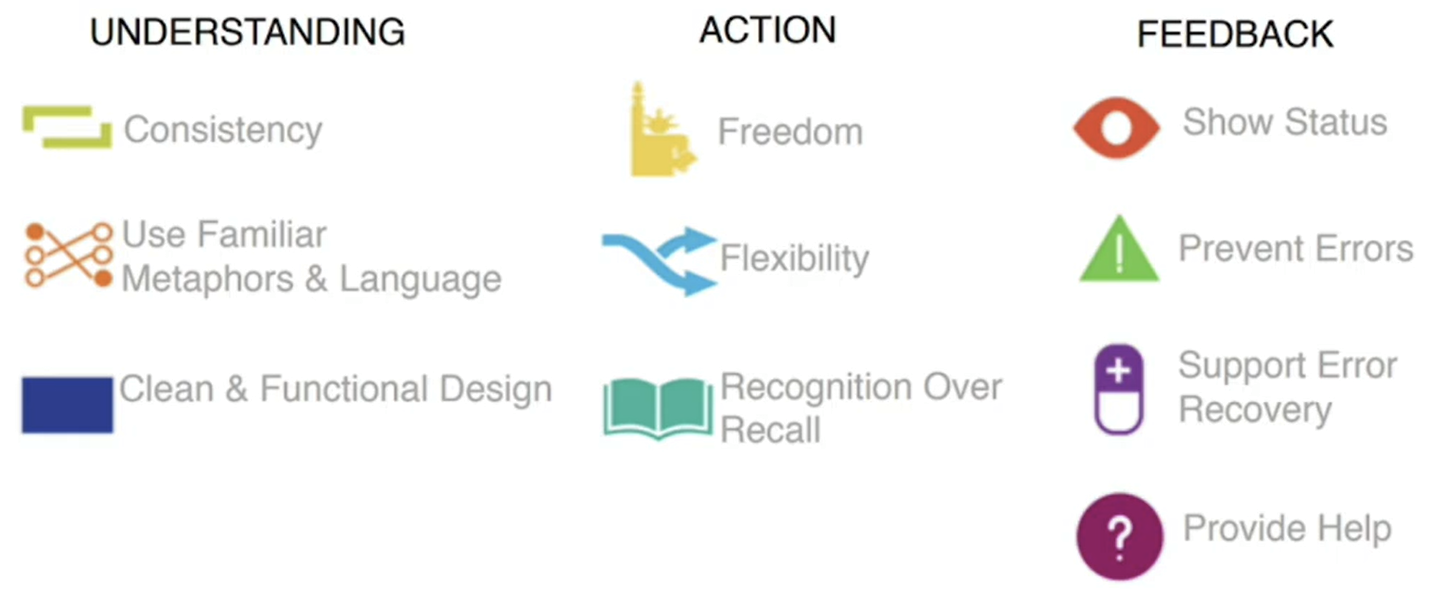
\includegraphics[width=0.5\linewidth]{Degree//static/SE_heuristic_summary.png}
        \caption{Design Heuristics Summary}
        \label{fig:ST-design-heuristic-summary}
    \end{figure}
    \item Importance of \href{https://www.vox.com/first-person/2017/3/1/14777110/typography-oscars-2017}{typography}.
\end{itemize}

\section{Project Estimation Techniques}
\subsection{Introduction}
\begin{itemize}
    \item \textbf{Importance of Estimation}: Establishing cost and Schedule. From a Client's perspective cost and schedule must be provided to them.
    \item \textbf{Key Estimation Parameters}: Size/Lines of code(KLOC, number of 1000 lines of code), Effort(How many people are required in the team, Person-month, effort an individual can typically put in a month).
    \item \textbf{Empirical Estimation}: Ask people who have completed similar projects.
    \item \textbf{Expert Judgment}: They can make an educated guess, but can encounter human errors, individual bias, optimistic estimates, overlook some factors, lack of adequate knowledge. To some extent, this can be averted by having a group of experts.
    \item \textbf{Delphi Technique}: Coordinator provides multiple Experts the SRS document and a form for recording cost estimates. Experts submit their estimates to the coordinator. Then the coordinator prepares a summary and distributes to all experts. Now, experts look at this summary and re-estimate the cost. This process can be iterated over several rounds.
    \item \textbf{Heuristic Technique}: Modelled using suitable mathematical expressions.
    \item \textbf{COCOMO Estimation Model}: Constructive Cost Estimation Model, $Effort=a\times SIZE^b$. $a$ and $b$ depend on the type of project.
    \item \textbf{Types of Projects}: Organic(Well understood application program, and team size is small and experiences), Semi-detached(Mix of experienced and inexperienced people), Embedded(Strongly couple with hardware).
    \item For Organic projects $a=2.4$ and $b=1.05$, for semi-detached project $a=3.0$ and $b=1.12$, and for embedded projects $a=3.6$ and $b=1.20$.
    \item \textbf{Effort Estimation Parameters}: People working on the project, Technical attributes of the project, Tools and practices used by the team.
    \item In COCOMO model, after getting initial estimates we add \textbf{cost driver attributes}. This would include Reliability, Database sizes, etc.
    \begin{figure}[H]
        \centering
        \begin{subfigure}[b]{0.40\textwidth}
            \centering
            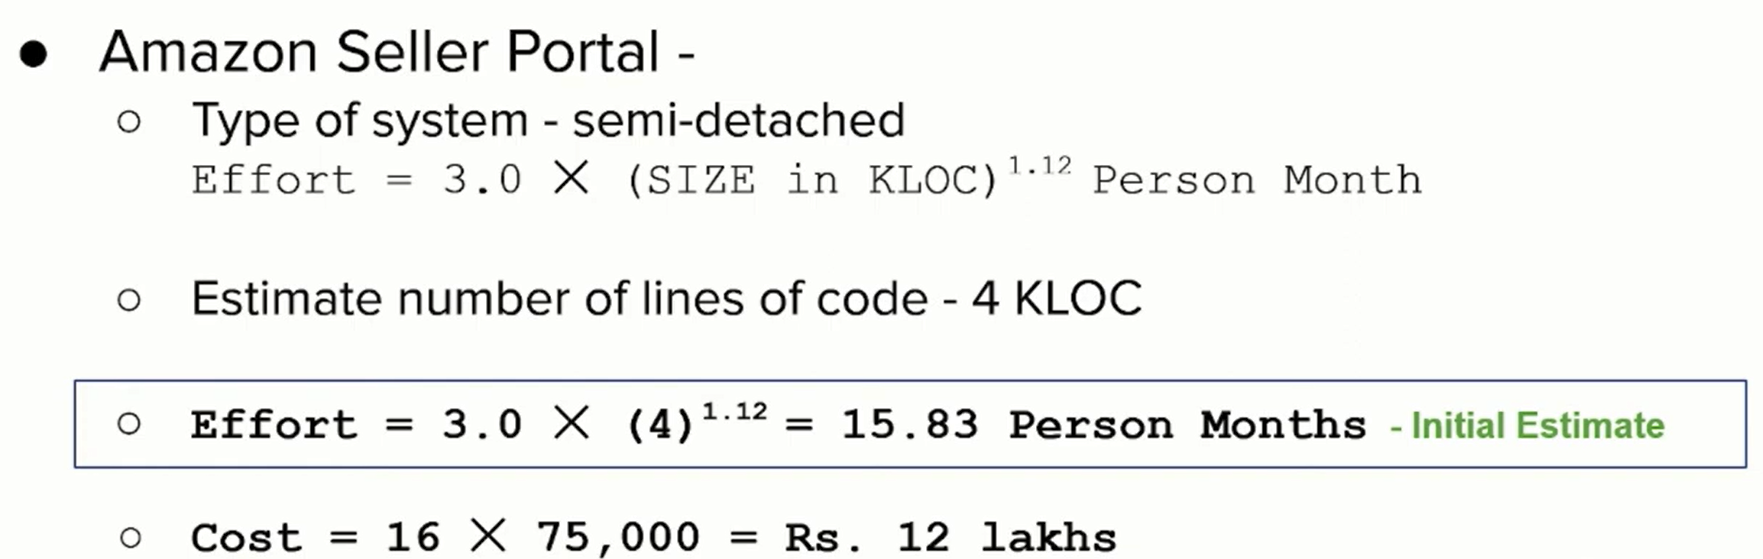
\includegraphics[width=\textwidth]{Degree/static/SE_COCOMO_ex.png}
            \caption{COCOMO model}
        \end{subfigure}
        \hfill
        \begin{subfigure}[b]{0.50\textwidth}
            \centering
            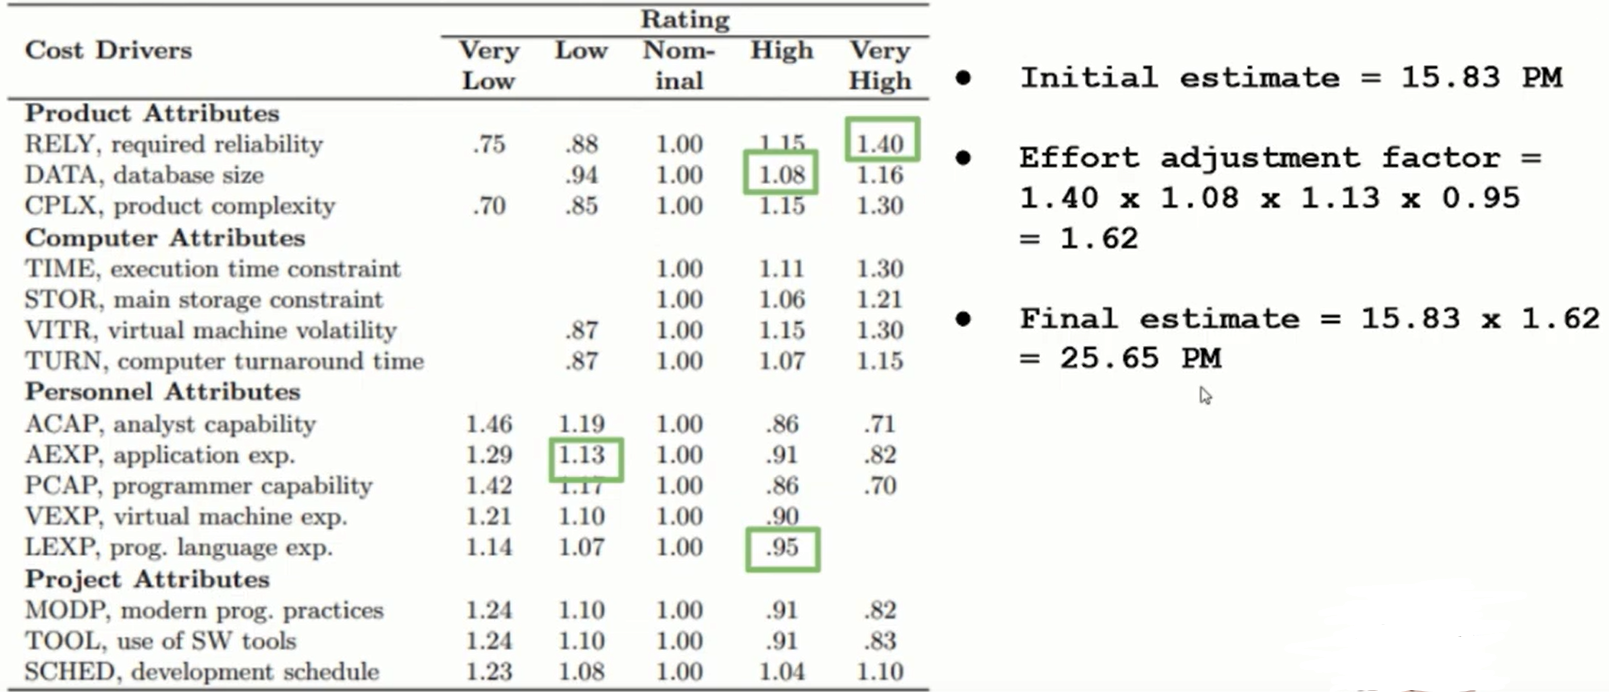
\includegraphics[width=\textwidth]{Degree/static/SE_cost_driver.png}
            \caption{Cost Drivers}
        \end{subfigure}
        \caption{Amazon Seller Portal Example}
        \label{fig:SE-amazon-seller}
    \end{figure}
\end{itemize}

\subsection{Project Scheduling}
\begin{itemize}
    \item Helps monitor timely completion of a task, and take corrective action if it falls behind.
    \item The Schedule can be built in steps as follows
    \begin{enumerate}
        \item Identify all major activities,
        \item Break down each activity into tasks,
        \item Determine the dependency among different tasks,
        \item Estimations for time durations required to complete the tasks,
        \item Represent this information in a chart/graph/network,
        \item Determine task starting and end dates from the representation,
        \item Determine the critical path(a chain of tasks that determine the duration of the project),
        \item Allocate resource to the tasks.
    \end{enumerate}
    \item Breakdown of activities can be done using \textbf{Work Breakdown Structure(WBS)}, it will create a tree like structure as follows
    \begin{enumerate}
        \item \textbf{Root}: Project name
        \item Each node is broken down into smaller activities, \textbf{children}
        \item Each leaf represents a task which can be allocated to a developer and scheduled.
        \item \textbf{Task}: Each task should take roughly two weeks to develop.
    \end{enumerate}
    \item Once we have the breakdown, now we create the activity network.
    \item \textbf{Activity Network}: Different activities making up a project, estimated durations, interdependencies. Leaf nodes of the WBS become the nodes of the activity network.
    \begin{figure}[H]
        \centering
        \begin{subfigure}[b]{0.45\textwidth}
            \centering
            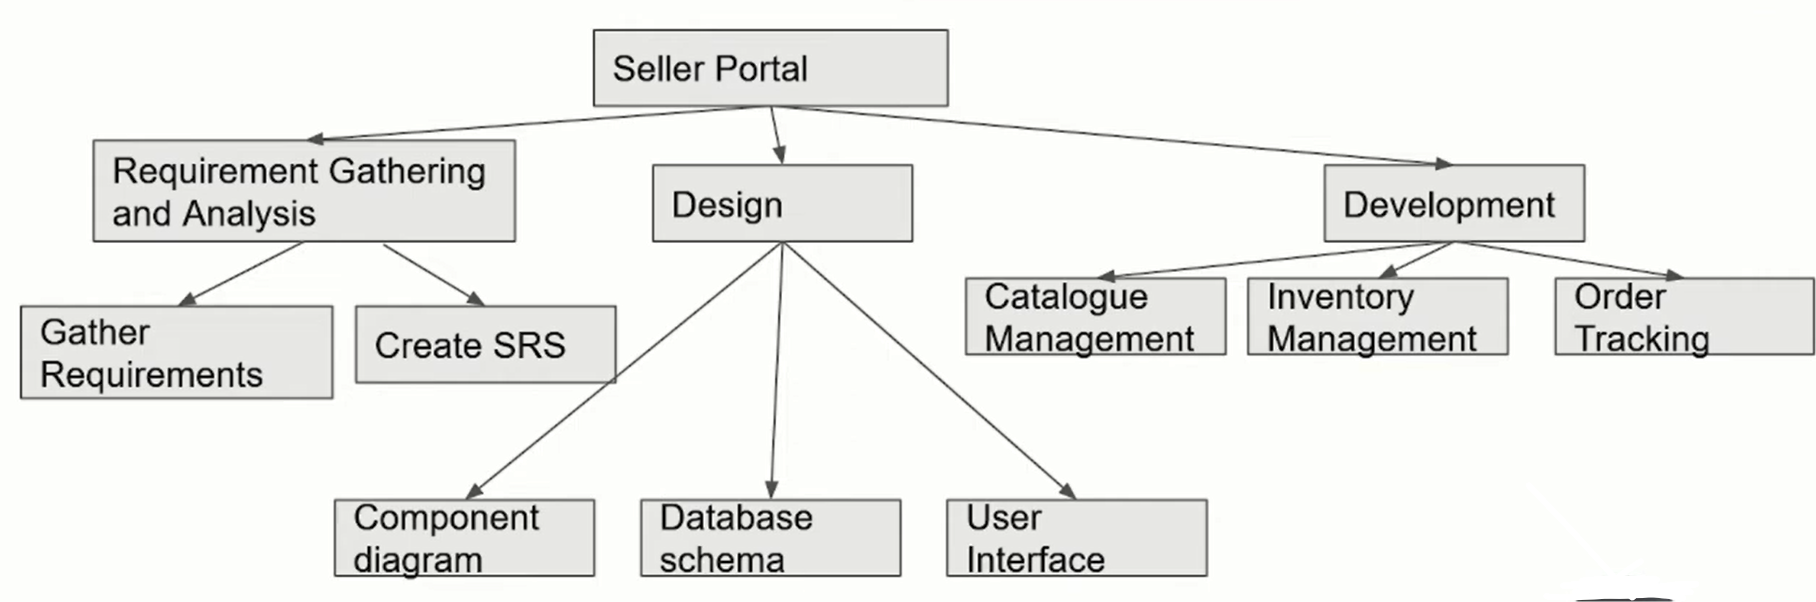
\includegraphics[width=\textwidth]{Degree/static/SE_Seller_WBS.png}
            \caption{Work Breakdown Structure}
        \end{subfigure}
        \hfill
        \begin{subfigure}[b]{0.45\textwidth}
            \centering
            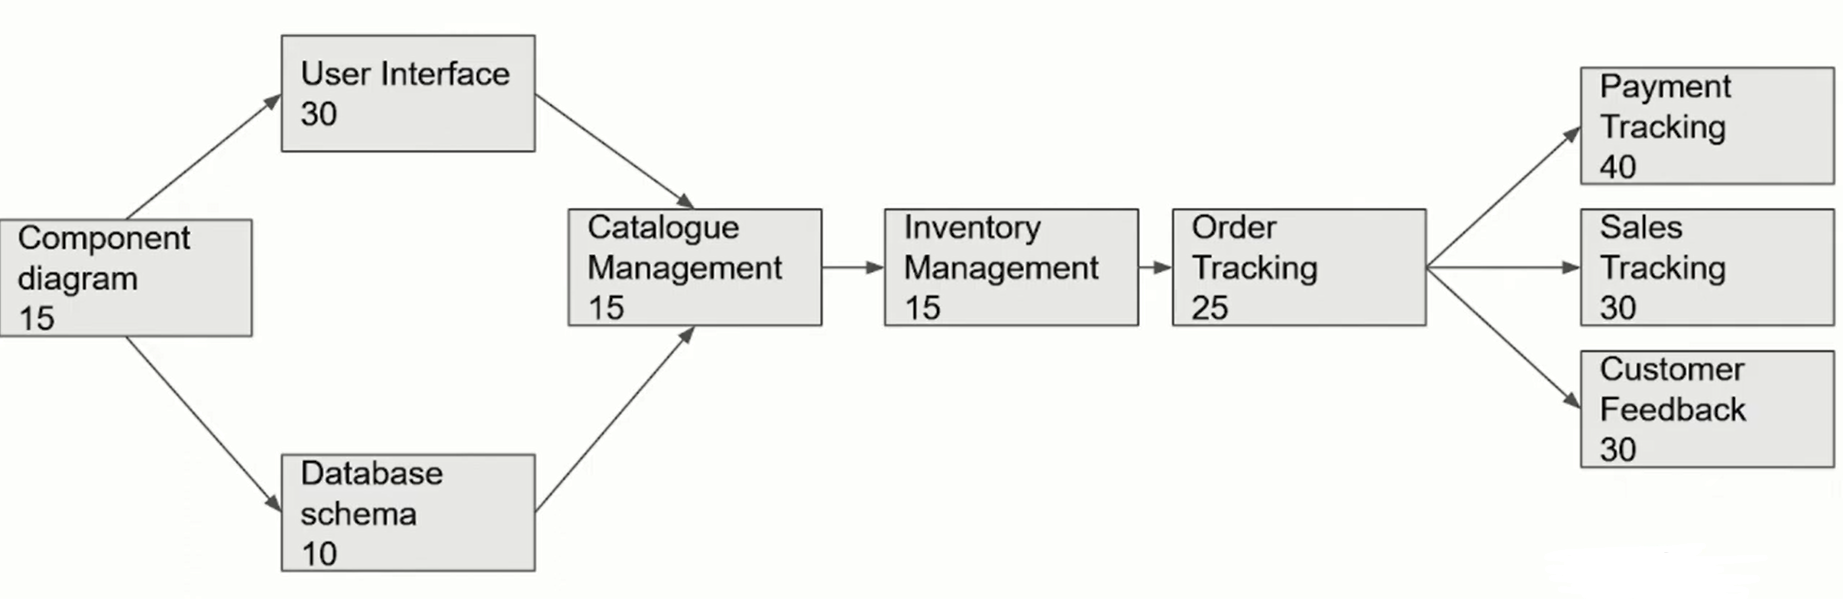
\includegraphics[width=\textwidth]{Degree/static/SE_Activity_Network.png}
            \caption{Activity Network}
        \end{subfigure}
        \caption{Seller Portal Example}
        \label{fig:SE-seller-portal}
    \end{figure}
    \item \textbf{Gantt Chart}: Another way to represent Activity network, it is a type of chart.
\end{itemize}

\subsection{Risk Management}
\begin{itemize}
    \item A risk is an anticipated unfavorable event or circumstance that can occur while a project is underway. This can be due to intangible nature of software, conflicts in a team.
    \item \textbf{Technical Risks}: Due to development team's insufficient knowledge about the product.
    \item Developing the wrong functions and user interfaces, can be mitigated by communicating with clients and build prototypes.
    \item Shortcomings in external components, can be mitigated by benchmarking and regular inspections.
    \item \textbf{Project Risks}: Project risks occur due to problems in budget, schedule, personnel, resources, and customer related problems.
    \item Most common type is schedule slippage, the project falls behind schedule, can be mitigated by creating detailed milestones, constant iterations, communicate frequently with clients.
    \item Insufficient domain knowledge/technical knowledge, can be mitigated by hiring developers with relevant experience, or we could outsource to third party vendors.
    \item Personnel shortfalls, can be mitigated by cross-training, train multiple people with skills required to work on the project.
    \item \textbf{Business Risks}: Risks which can harm the business aspects of the software product.
    \item Product is no longer competitive in the market, can be mitigated by exploring the market for similar products.
    \item Gold plating, developing unnecessary features, can be mitigated by communicating with clients and do cost-benefit analysis.
    \item \textbf{Risk Assessment}: Project manager asks everyone in the team for worst case scenario and the PM then creates a "risk table".
    \item Then a probability(P) is assigned to each risk, each risk is also assigned Impact(I), which can negligible, marginal, critical, catastrophic(1-4).
    \item The risk is then calculated as $Risk=P\times I$, which then is sorted in descending order and decide which risk need to mitigated first.
\end{itemize}

\subsection{Project Management in Agile}
\begin{itemize}
    \item Does not predict cost and schedule at the start of the project.
    \item \textbf{Team formation}: Usually team size is 4–9 people, and we organize development using \textbf{Scrum}. At the heart of scrum are sprints.
    \item \textbf{Sprint}: short, time-boxed period when a scrum team works to complete a set amount of work.
    \item \textbf{Development Team}: Whoever is required to complete work in that given sprint.
    \item \textbf{Product Owner}: Interfaces between the client and the development team.
    \item \textbf{Scrum Master}: Ensures all activities are being done well.
    \item \textbf{Sprint Planning}: This is a collaborative event between product owner, scrum master, and the development team. We ask two basic questions, What work can get done in this sprint? and How will the chosen work get done?. This meeting is roughly 2 hours per week of its iteration.
    \item \textbf{Product Backlog}: Prioritized list of work for the development team that is derived from user stories and requirements. Prioritizing will be done in sprint planning meetings.
    \item \textbf{Standup/Daily Scrum Meeting}: Daily meeting which involves everybody. Each member answers three questions, What did I work on yesterday?, What am I working on today?, and What issues are blocking me?
    \item \textbf{Sprint Review}: After the sprint the team demonstrates what they have completed. Move things from To-Do, In Progress to Done.
    \item \textbf{Sprint Retrospective}: Evaluate the last sprint, Discuss user stories/tasks that went well/didn't go well, and finally create and implement a plan.
    \item \textbf{Project Scheduling}: Key indicator of progress is how many user stories are implemented. Project estimation can be simply counting the number of user stories completed per iteration/sprint.
    \item Not all user stories require the same effort, and hence this can lead to mis-prediction. This is mitigated by assigning points to user stories, and calculate \textbf{velocity} which is the number of points per iteration/sprint.
    \item One good software to do this is \textbf{Pivotal Tracker}, Link for which can be found \href{https://www.pivotaltracker.com/}{here}.
\end{itemize}

\section{Software Design}
\subsection{Outcomes of the Design Process}
\begin{itemize}
    \item We will design an high level view of software architecture
    \begin{enumerate}
        \item \textbf{Components}: Collection of functions and data, should accomplish some well-defined tasks.
        \item \textbf{Interfaces}: How components communicate with each other.
        \item \textbf{Data Structures}: Suitable data structures for storing and managing data.
        \item \textbf{Algorithms} required to implement individual components.
    \end{enumerate}
    \item Characterizing a Good Software Design
    \begin{enumerate}
        \item \textbf{Correctness}: Correctly implement all the functionalities of the system.
        \item \textbf{Efficiency}: Ensure that resources, time, space, cost, are managed well.
        \item \textbf{Maintainability}: Easy to Change
        \item \textbf{Understandable} by everyone in the development team.
    \end{enumerate}
\end{itemize}

\subsection{Design Modularity}
\begin{itemize}
    \item When all functions in a module perform a single objective, the module is said to have good cohesion.
    \item \textbf{Coupling}: Measure of the degree of interaction between two modules.
    \item \textbf{Cohesion}: Measure of how functions in a module cooperate together to perform a single objective.
    \item A good design will have high cohesion and low coupling.
    \item \textbf{Modular}: Problem has been decomposed into a set of modules that have only limited interactions with each other.
    \item \textbf{High cohesion}: Functions of the module cooperate with each other for performing a single objective.
    \item Two modules are \textbf{data coupled} if their communication is using a primitive data type.
    \item \textbf{Control Coupling}: Data is passed that influence the internal logic of a module.
    \item \textbf{Common Coupling}: If two modules share global data items.
    \item \textbf{Content Coupling}: If one module refers to the internals of the other module.
    \item \textbf{Functional Cohesion}: Different functions of the module cooperate to complete a single task.
    \item \textbf{Sequential Cohesion}: Different functions of the module execute in a sequence. Output from one function is input to next in the sequence.
    \item \textbf{Communicational Cohesion}: If all functions of the module refer to or update the same data structure.
    \item \textbf{Procedural Cohesion}: Activities in the module are related by sequence. Set of functions in the module are expected one after the other, work towards entirely different purposes.
    \item \textbf{Coincidental Cohesion}: Module has functions with meaningless relationships with one another.
\end{itemize}

\subsection{Object-Oriented Design}
\begin{itemize}
    \item \textbf{Object} are key building blocks. Working of a software in terms of interacting objects. Usually represent a tangible real-world entity.
    \item An object contains data, methods, and they follow encapsulation. This ensures data hiding/abstraction.
    \item \textbf{Class} are template for object creation. All objects possessing similar attributes and methods constitute a class.
    \item \textbf{Association}: Take each other's help to perform some functions.
    \item \textbf{Composition}: Represents whole/part relationships.
    \item \textbf{Inheritance}: Extend features of an existing class.
    \item \textbf{Dependency}: If class B depends on class A, if any changes are made to class A, changes have to be made to class B as well.
\end{itemize}

\subsection{Unified Modelling Language Diagrams}
\begin{itemize}
    \item \textbf{Modelling}: Creating an external, explicit representation of the system to be built.
    \item \textbf{UML} help represent the software design via multiple views and greater level of detail.
    \item \textbf{Structural View}: Structure/components of the software system, and relationships. It describes logical parts of the system, i.e., classes, data, and functions.
    \item \textbf{Class Diagram}: Describes the structure of the system. Describes the system's classes, attributes, operations, relationships among objects.
    \item \textbf{Dynamic Behavioral View}: Describes behavior of the system over time. Further classified into
    \begin{enumerate}
        \item \textbf{State Machine View}: Models different states of an object of a class.
        \item \textbf{Activity View}: Models flow of control among computational activities.
        \item \textbf{Interaction View}: Sequence of message exchanges among parts of a system.
    \end{enumerate}
    \begin{figure}[H]
        \centering
        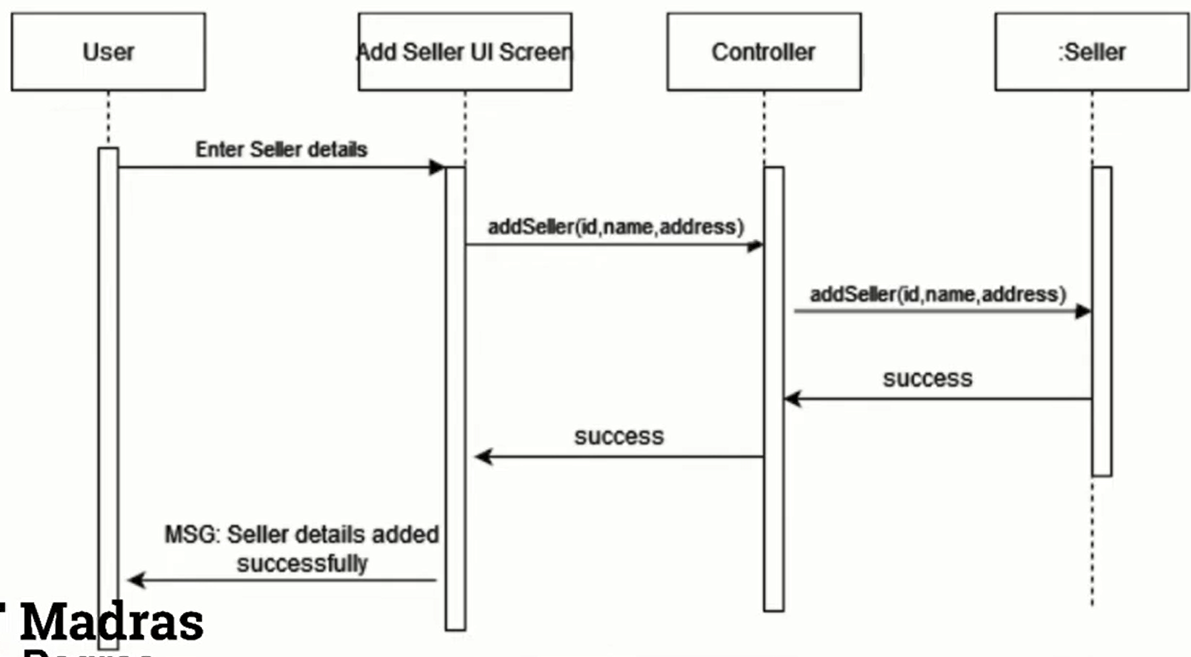
\includegraphics[width=0.8\linewidth]{Degree//static/SE_sequence_diagram.png}
        \caption{Sequence Diagram for adding seller using Interaction View}
    \end{figure}
    \item \textbf{Purposes of Modelling}
    \begin{enumerate}
        \item Serves as a vehicle for communication and idea generation.
        \item Guide Development of software
        \item Close correspondence with the implementation. Generate code from models.
    \end{enumerate}
    \item \textbf{VeriSIM}: \textbf{Veri}fying designs by \textbf{Sim}ulating Scenarios. Develop an integrated understanding of class and sequence diagrams. A VeriSIM learning platform can be found \href{https://verisim.tech/}{here}.
    \item \textbf{Design Tracing Strategy}: Construct a state diagram which models the scenario.
    \item Check chapter 3 of the reference manual for an overview, it can be found \href{https://drive.google.com/file/d/1Jd-X3rmu4JLpsZgn1dPV7AFo-NGsFi3H/view}{here}.
    \begin{figure}[H]
        \centering
        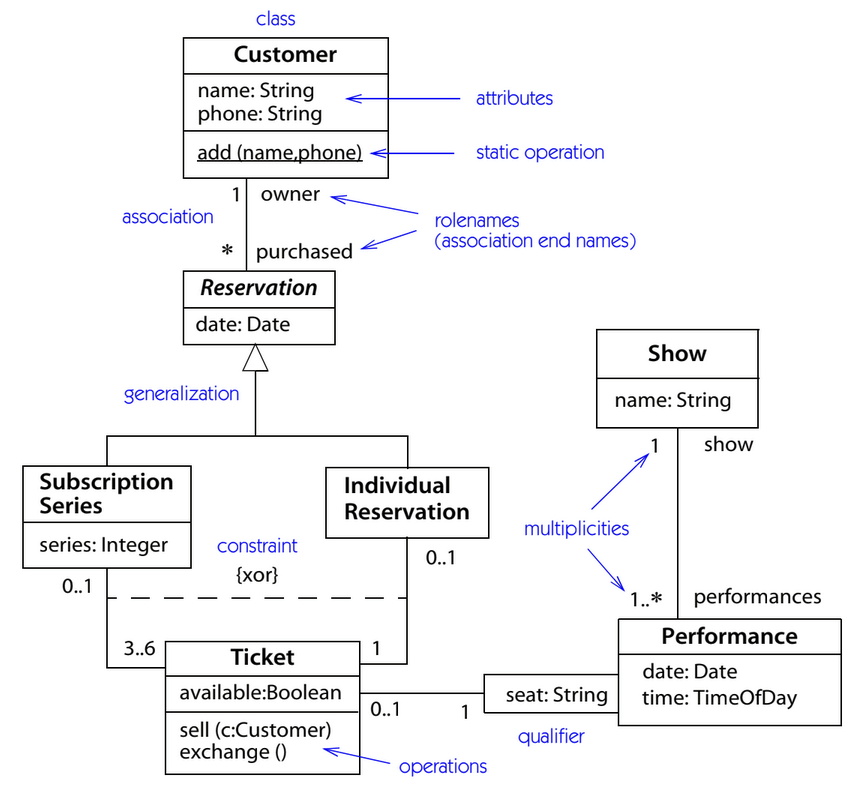
\includegraphics[width=0.55\linewidth]{Degree//static/SE_class_diagram.png}
        \caption{UML Class Diagram}
    \end{figure}
\end{itemize}

\section{Software Development}
\subsection{Rest APIs}
\begin{itemize}
    \item Use $editor.swagger.io$, can be found \href{https://editor.swagger.io/}{here}.
    \item Use Insomnia software for testing downloaded YAML file and code. Download link can be found \href{https://insomnia.rest/download}{here}.
\end{itemize}

\subsection{Version Control System}
\begin{itemize}
    \item Several developers are working on a project. One developer changed some code that caused a failure and now the system cannot start. Either\\
    Identify and fix the issue. Could take a long time to debug as you don't know the change history, till then no other team member can test their new code changes as the bug will not let the system start.\\
    Or just roll back to the previous version of code that was running stable.
    \item Consider a company with hundreds of clients of a software system. Every client specific feature needs a new version to be released and maintained.\\
    Huge code vase, code duplicated.\\
    Several versions result in multiple copies of code. Difficult to maintain and administer these copies manually.
    \item \textbf{VCS}: A system that helps in tracking and managing changes to the \textbf{source code} or other documents, and maintaining versions of the code.
    \item Increases productivity, Better communication and collaboration, Saving space on multiple revisions through diffs/snapshots, Better efficiency even as teams scale.
    \item \textbf{Centralized VCS}: maintained on the server, that everybody shares. Entirely based on client server model. Checkout whole or part of the repository, make changes and push back the changes to the server. Highly dependent on the server.\\
    Anything goes wrong, the development halts till the server is up again.\\
    May even lose entire history or repository if no backups configure.
    \item \textbf{Distributed VCS}: Entire repository is mirrored locally that includes the full change history. Centralized repository hosting possible but complete dependency is not on it. Basically everyone owns their own local copies of the repository.
    \item \textbf{Git}: Free and open source VCS. Focus is on speed, data integrity and working on multiple tasks.
    \item \textbf{Modified}: After you change the file in your working directory.
    \item \textbf{Staged}: You marked the file to be committed.
    \item \textbf{Committed}: Changed stored in the local database. But only the staged files will be committed.
    \item \textbf{Create a new repository}: \textit{git init} initializes a new git repository in your current working directory. \textit{git add filename} stage the modified files. \textit{git commit -m "change description"} commit the staged files to DB.
    \item \textbf{Clone a repository}: \textit{git clone url local directory} mirror repo located at "url" to "local directory".
    \item \textit{git push} to push changes to the remote repo.
    \item \textit{git pull} fetch and download changes from remote rep and update local repo.
    \item \textit{git status} view the status of your local files in the working directory and staging area.
    \item \textit{git diff} show changes between commits, commit and working tree
    \item \textit{git reset HEAD filename} unstage the file
    \item \textit{git checkout filename} undo the changes that are committed but not yet pushed to remote.
    \item \textit{git log} check commit logs/history.
    \item \textbf{Branching}: Branches are independent versions of repository. Mechanism to diverge work from the main project line.\\
    \textit{git branch feature1} create a new branch named feature1 from the base branch you are working on.\\
    \textit{git branch} list all local branches\\
    \textit{git checkout} command to switch branch, \textit{git checkout feature1}
    \item \textbf{Merging}: A way to combine changes made through one or more branches to a single branch.\\
    \textit{git merge feature1} merge the branch "feature1" to the current working branch.
    \item \textbf{Rebase}: Incorporate changes from one branch to another. Incorporate latest changes from master branch to feature1 branch. \textit{git rebase}.
    \item For more details refer git-scm book, can be found \href{https://git-scm.com/book/en/v2}{here}.
    \item An issue is reported by developer or tester or user when encountered, this needs to be saved and tracked till it is fixed. We need a system to do this.
    \item Can create a branch or pull request to map to an issue. Can map more than one issues to a branch.
    \item \textbf{Code Reviewing}: Quality assurance in which multiple people examine the changes done by a developer.
    \item Improves code Quality, Focus not just on correctness but also on aspects like efficiency, complexity and security.
    \item Minimize Technical debt, Well documented code with consistent design and implementation reduces maintenance costs and efforts.
    \item Risk reduction, Testing cannot guarantee software to be completely bug free.
    \item Supports Knowledge transfer, Learn from others expertise.
    \item Make QA testing easier, Many risks can be identified at earlier stage itself.
    \item \textbf{Pair programming}: An agile software development technique in which two programmers work together at one workstation. One writes code while the other reviews the code. The two programmers switch roles frequently. Getting popular slowly.
\end{itemize}

\subsection{Debugging}
\begin{itemize}
    \item \textbf{Error}: discrepancy between actual behaviour and intended behaviour
    \item \textbf{Failure}: Observable error, Incorrect output value, exception etc.
    \item \textbf{Fault}: Where the failure has occurred (lines in code)
    \item \textbf{Debugging}: determining the cause of failure
    \item Reproduce the problem $\to$ Find cause of defect $\to$ Investigate fix $\to$ Implement fix $\to$ Test fix
    \item \textbf{Logging}: insert print statements
    \item \textbf{Dump \& diff}: use diff tool to compare logging data between executions
    \item \textbf{Stepping in debugger}
    \item \textbf{Profiling tool}: how often, how long various parts of program are executed.
    \item \textbf{Input manipulation}: Edit inputs, observe differences in output
    \item \textbf{Backwards}: Find statement that generated incorrect output, follow data and control dependencies backwards to find incorrect line of code
    \item \textbf{Forwards}: Find event that triggered incorrect behavior, follow control flow forward until incorrect state reached
    \item \textbf{Black box debugging}: Find documentation, code examples to understand correct use of API
    \item Pdb: Python Debugger
\end{itemize}

\subsection{Software Metrics}
\begin{itemize}
    \item Quantitative way to measure the quality of your code
    \item \textbf{Cyclomatic Complexity}: Number of decisions a block of code contains $+ 1$, use \textit{Radon}(python package).
    \begin{figure}[H]
        \centering
        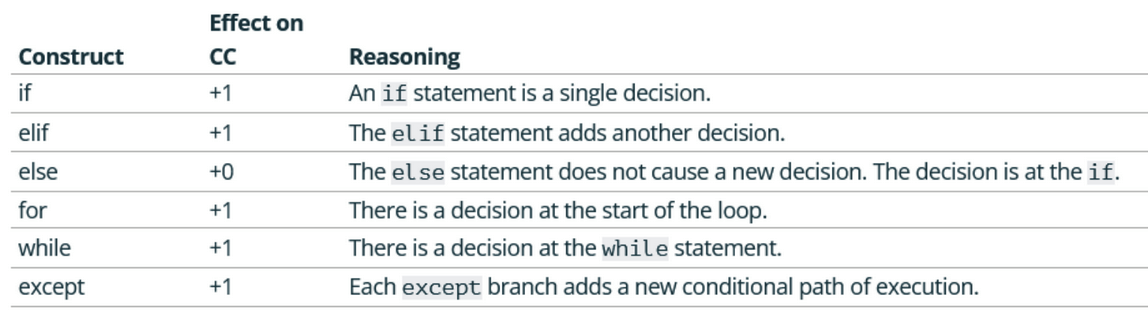
\includegraphics[width=\linewidth]{Degree//static/SE_Cyclomatic_complexity.png}
        \caption{Cyclomatic Complexity effects}
    \end{figure}
    \begin{figure}[H]
        \centering
        \begin{subfigure}[b]{0.45\linewidth}
            \centering
            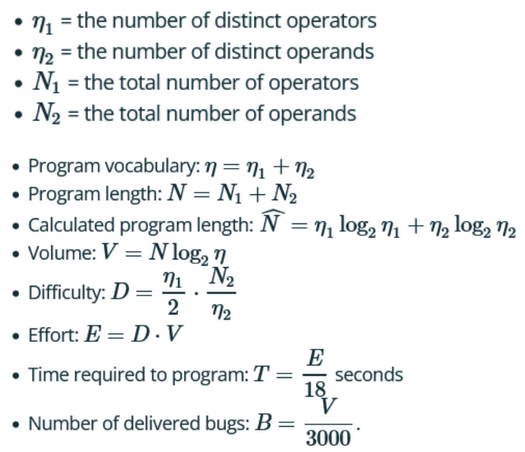
\includegraphics[width=0.7\textwidth]{Degree//static/SE_Halstead_metrics.png}
            \caption{Halstead's Metrics}
        \end{subfigure}
        \hfill
        \begin{subfigure}[b]{0.45\linewidth}
            \centering
            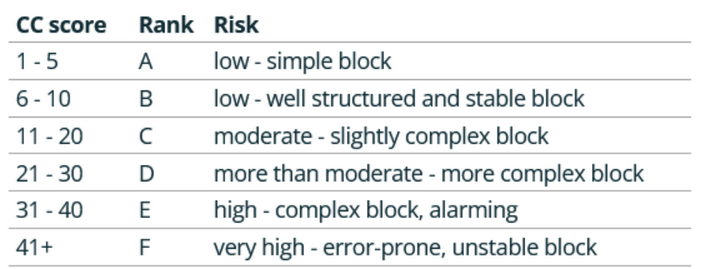
\includegraphics[width=\linewidth]{Degree/static/SE_CC_score.png}
            \caption{CC Score}
        \end{subfigure}
    \end{figure}
    \item \textbf{LOC}: The total number of lines of code.
    \item \textbf{LLOC}: The number of logical lines of code. Every logical line of code contains exactly one statement
    \item \textbf{SLOC}: The number of source lines of code
    \item \textbf{Comments}: The number of comment lines
    \item \textbf{Code Smells}: Certain problematic characteristics in a code
    \item Redundant comments, Commented out code
    \item Functions doing more than one thing, Functions that are too long, Functions having too many arguments, Functions having flag arguments, Dead functions
    \item \textbf{Don’t repeat yourself (DRY)}: Clumps of identical code throughout the program, Put this code in simple methods, Incorrect behaviour at the boundaries, Use explanatory variables
    \item \textbf{Refactoring}: Changing the code by improving its structure, without changing its behaviour.
\end{itemize}

\section{Software Architecture}
\subsection{Introduction}
\begin{itemize}
    \item Way of organizing your code
    \item Define software elements/modules, relations among them, and properties of both elements and relations.
    \item \textbf{Client-server systems}: data is transacted in response to requests
    \item \textbf{Pipe and filter}: data is passed from component to component, and transformed and filtered along the way
    \item \textbf{Model-view-controller}: Architectural style where views of the data are separated from the manipulations of data
    \begin{enumerate}
        \item \textbf{Model}: the component which models the data required for the service
        \item \textbf{View}: the GUI objects, presentation layer, visual representation of the Model
        \item \textbf{Controller}: coordinates multiple Views on the screen, and helps users manipulate the model
    \end{enumerate}
    \item \textbf{Peer to Peer Architecture}: Distributed application - different systems form nodes, and share resources with each other. 
    \item No centralized system which monitors all transactions of the system
    \item Nodes in the network make processing power, disk storage etc. directly available to other nodes in the network
    \item \textbf{Component}: A well-defined functionality or behavior separate from other functionality and behavior
    \item \textbf{Connectors}: Code that transmit information between components. Responsible for regulating interactions between components
    \item \textbf{Protocols}: Set of pre-defined rules which describe how components should interact with each other
    \item \textbf{Design Patterns}: Descriptions of communicating objects and classes that are customized to solve a general design problem in a particular context
    \item \textbf{Design Smells}: warning signs that your code may be heading towards an antipattern
    \item \textbf{SOLID Guidelines}: Avoid design smells
    \item \textbf{Refactoring}: moving code between classes, creating new classes or modules, removing classes that aren’t required
\end{itemize}

\subsection{SOLID Principles}
\begin{itemize}
    \item Object-oriented principles for software design, Makes code easy to understand, modular
    \begin{enumerate}
        \item \textbf{S}: Single Responsibility Principle, Every class has a single responsibility/purpose
        \item \textbf{O}: Open-Closed Principle, Software entities should be open for extension, but closed for modification
        \item \textbf{L}: Liskov Substitution Principle, Derived classes should be substitutable by their base class
        \item \textbf{I}: Interface Segregation Principle, Specify what the interface should do, not how.\\
        "do not force any client to implement an interface which is irrelevant to them"
        \item \textbf{D}: Dependency Inversion Principle, Prefer abstraction/interfaces over implementations
    \end{enumerate}
\end{itemize}

\subsection{Design Patterns}
\begin{itemize}
    \item Design patterns are descriptions of communicating objects and classes that are customized to solve a general design problem in a particular context. 
    \item \textbf{Problem}: When to apply the design patterns, in what context
    \item \textbf{Solution}: Describe the elements that make up the design, their relationships, responsibilities and collaborations. Essentially make a template that can be applied in many different situations.
    \item \textbf{Creational}: Used during the process of object creation
    \begin{enumerate}
        \item \textbf{Factory Design Pattern}: Replace object construction calls with calls to a special factory method.\\
        \textbf{Pros}: Single Responsibility Principle, Open-Closed Principle\\
        \textbf{Cons}: Code may become more complicated, a lot of new subclasses needed to implement the pattern
        \item \textbf{Builder Design Pattern}: Optional parameters necessitates use of multiple constructors, this is known as telescoping constructors.\\
        \textbf{Solution}: move object construction code it to separate objects called builders\\
        \textbf{Pros}: Construct objects step by step, Single Responsibility Principle\\
        \textbf{Cons}: Code may become more complicated, new classes, methods need to be created
    \end{enumerate}
    \pagebreak
    \item \textbf{Structural}: Composition of classes or objects
    \begin{enumerate}
        \item \textbf{Facade Design Pattern}: Reusing code, will have to know details about different objects, functions\\
        \textbf{Solutions}: Provides a simple interface to a library, or a complex set of classes\\
        \textbf{Pros}: Isolate code from other libraries/classes’ complexity\\
        \textbf{Cons}: Tightly coupled to other objects, maintenance becomes more difficult
        \item \textbf{Adapter Design Pattern}: Some products have cost in dollars/euros. Conversion to rupees is needed\\
        \textbf{Pros}: separate data conversion code from primary business logic, New types of adapters\\
        \textbf{Cons}: Overall code complexity increases
    \end{enumerate}
    \item \textbf{Behavioral}: Characterize the ways in which classes or objects interact and distribute responsibility
    \begin{enumerate}
        \item \textbf{Iterator Design Pattern}: Different types of collections, How to access and iterate through elements?\\
        \textbf{Solution}: Separate the behaviour of how elements are accessed into a separate object called an iterator\\
        \textbf{Pros}: Separate access of elements from other functionalities, new types of iterators, collections\\
        \textbf{Cons}: Can be an overkill for simple collections
        \item \textbf{Observer Design Pattern}: Notify a particular set of buyers when a new product is launched\\
        \textbf{Solution}: Subject object maintains a list of observers, Notifies them of automatically of any changes
        \item \textbf{Strategy Design Pattern}: Process orders based on different strategies\\
        \textbf{Solution}: Extract different strategies (algorithms) into separate classes, Original class (context) delegates the work to strategy object\\
        \textbf{Pros}: Isolate implementation details of algorithm, new strategies without changing existing classes\\
        \textbf{Cons}: Not required if there are only a few algorithms which will be used
    \end{enumerate}

\end{itemize}

\section{Testing}
\subsection{Motivation}
\begin{itemize}
    \item Errors in software programs, even simple errors can cause entire systems to crash.
    \item \textbf{Test case}: triplet $[I,S,R]$\\
    I: data input to the programming\\
    S: State of the program at which the data is to be input\\
    R: result expected to be produced by the program
    \item \textbf{Test suite}: Set of all test cases which have been designed to test a given program.
    \item Testing for a large collection of randomly selected test cases do not guarantee that all errors will be uncovered.
    \item Domain of all input values in a software system is sufficiently large.
    \item Necessary to design a minimal test suite where each test case helps detect different types of errors.
    \item \textbf{Unit testing}: Individual functions/units of a program are tested.
    \item \textbf{Integration testing}: Units are incrementally integrated and tested after each step of integration.
    \item \textbf{System testing}: the fully integrated system is tested
    \item \textbf{Alpha testing}: test team within the organization
    \item \textbf{Beta testing}: select group of customers
    \item \textbf{Acceptance testing}: customer to determine whether to accept the delivery of the software.
\end{itemize}

\subsection{Unit Testing}
\begin{itemize}
    \item While testing a module, other modules with which this module needs to interface may not be ready.
    \item Makes debugging easier.
    \item When: During the coding of the module. Not in the testing phase
    \item Who: Person writing the code for the module.
    \item Python unit testing: \textit{unittest} and \textit{pytest}
\end{itemize}

\subsection{Black box and White box testing}
\begin{itemize}
    \item \textbf{Black box testing}: Examining input/output values only, No knowledge of design or code required
    \item \textbf{Equivalence Class Partitioning}: Domain of input values partitioned into a set of equivalence classes. Program behaves similarly for every input data in a particular equivalence class.
    \item \textbf{Boundary Value Analysis}: Examine the values at boundaries of the equivalence classes.
    \item \textbf{White box testing}: Analyze the structure of the program using some heuristics
    \item \textbf{Branch coverage}: Every branch in the program needs to be taken at least once
    \item \textbf{Multiple branch coverage}: Each component condition takes true and false values
    \item \textbf{Path coverage}: access all linearly independent path at least once.
\end{itemize}

\subsection{Integration and System testing}
\begin{itemize}
    \item When at least a few or all modules have undergone unit testing
    \item \textbf{Integration testing}: detect errors at the module interfaces
    \item \textbf{Big Bang Approach}: All modules integrated in a single step
    \item \textbf{Bottom up Approach}: Modules of each sub system are integrated, Not necessary to create stubs, Drivers are required.
    \item \textbf{Top-down Approach}: Starts with the root module + 1-2sub-ordinate modules of the root module, Stubs are required.
    \item \textbf{Mixed Approach}: Use both top-down and bottom-up testing
    \item \textbf{Smoke testing}: Carried out before initial system testing, Checking whether basic functionalities are working, Few basic test cases designed
    \item \textbf{Performance testing}: Check whether the system meets non-functional requirements
\end{itemize}

\subsection{Test Driven Development}
\begin{itemize}
    \item Used especially in Agile Processes
    \item Write tests first for the functionality that we want to implement
    \item Drive design and development of that functionality from tests
    \item Express the functionality/feature/requirement in the form of a test
    \item Create a test Run the test - See it FAIL
    \item Create the Minimum code to meet the needs of the test
    \item Run it and See it PASS
    \item REFACTOR code - quality, make it modular, more elegant
\end{itemize}

\section{Software Deployment}
\subsection{Development Environment and Strategies}
\begin{itemize}
    \item \textbf{Development Environment}: Local environment of a software developer, Contains IDE and other tools
    \item After Development or during we have a testing environment.
    \item \textbf{Staging Environment}: Exactly resembles the production environment, Run on a remote machine
    \item Deploying a software system involves a lot of activities, configurations etc.
    \item Staging helps Preview new features, Performance testing
    \item After staging, we push it to production environment.
    \item \textbf{Blue/Green Deployment}: Staged Deployment, Create a new separate production environment for the new version, without affecting the current one, Regular cycling between real and previous versions\\
    \textbf{Advantage}: rollback is easy
    \item \textbf{Canary Deployment}: Phased Rollout/Incremental Rollout, Slowly roll out the change to a small subset of users\\
    \textbf{Drawback}: manage multiple instances at once
    \item \textbf{Versioned Deployment}: Allow users to choose version, Keep all versions alive, If user updates, route them to the new version\\
    \textbf{Drawback}: have to maintain multiple versions
\end{itemize}

\subsection{Deployment Hosting}
\begin{itemize}
    \item Infrastructure required to host applications, Usually hosted on server systems
    \item no unplanned downtime
    \item \textbf{Bare Metal Servers}: Purchase actual server hardware, Server - CPU, motherboard, RAM, disk\\
    \textbf{Advantage}: highest performance\\
    \textbf{Disadvantage}: Most expensive upfront, Time, effort in setting up, maintenance
    \item \textbf{Infrastructure-as-a-service(IaaS)}: IaaS provider provides a part of the infrastructure\\
    \textbf{IaaS examples}: Digital Ocean, AWS, Linode\\
    \textbf{Advantages}: Cheaper, No maintenance overhead\\
    \textbf{Disadvantages}: Each IaaS has its own set of configurations, Shared by others so performance may suffer
    \item \textbf{Platform-as-a-Service(PaaS)}: Provides a software layer as well on which a web app can be deployed\\
    \textbf{Examples}: Heroku, Google App Engine\\
    \textbf{Advantage}: very easy to deploy \\
    \textbf{Disadvantage}: lack of control
\end{itemize}

\subsection{Continuous Integration}
\begin{itemize}
    \item Automating the integration and deployment of software
    \begin{enumerate}
        \item Developer commits code to version control system
        \item Continuous Integration Server pulls the new code
        \item CIS build and tests the new code
        \item Once code passes all tests, CIS signals Staging/Deployment server
        \item Staging server pulls the code from version control system
        \item Then it builds, tests, and deploys the new code.
        \item Once deployed Staging server signals back to CIS, and the process starts again.
    \end{enumerate}
    \item Maintain a single source repository
    \item Automate the Build, Build Tools: Ant, Gradle, Builder
    \item Make the Build Self-Testing, Create automated tests, When a test fails send notification to the developer
    \item Commit to the main branch everyday
    \item Infrequent commits can have increased chances of more conflict errors
    \item Frequent commits encourage developers to break down their works into very small chunks
    \item Every commit should build the main branch on an integration server
    \item \textbf{Continuous Integration Servers}: Jenkins, Cruise Control
    \item Fix broken builds immediately, take the system back to the last-known good build
    \item Write Scripts to automate deployment
    \item Benefits of Continuous Integration
    \begin{enumerate}
        \item Reduces deployment time, Avoids last-minute confusion and rush at release dates
        \item Beneficial to users, Can see an initial prototype
        \item Beneficial for developers, pushes developers to create modular code
    \end{enumerate}
    \item However, Initial effort required to setup processes
\end{itemize}

\subsection{Performance and Monitoring}
\begin{itemize}
    \item \textbf{Caching}: Store results of common operations in memory, Fetch from memory instead from database, examples include Memcached, Redis
    \item Different levels of caching are Web browser, Web server(page cache), Database query cache, results of recent queries which haven’t changed
    \item \textbf{Asynchronous work queue}: executed outside the HTTP request-response cycle
    \item Consists of Queue of jobs to be performed, parameters and Pool of workers take multiple jobs from queue
    \item Quick loading of pages is important, minifying code helps, and compressing static pages.
    \item Issues can still arise in the live environment
    \item \textbf{Generate reports}: Analyze page resources, find optimization suggestions, check SEO and accessibility metrics and calculate your performance score. One example of this is Lighthouse.
    \item \textbf{Clickstreams}: which sequences of pages do your users visit the most
    \item \textbf{Think time/dwell time}: how long does a typical user stay on a given page
    \item \textbf{Abandoment}: Check various flows in your application
    \item Embed a small piece of JS in every page on your site
    \item In canary deployment, check which version is better.
\end{itemize}

\section{Other Aspects}
\subsection{Software Organizations}
\begin{itemize}
    \item \textbf{Marketing Team}: Look for opportunities in the market, to provide value, Conduct market research, identify audiences
    \begin{figure}[H]
        \centering
        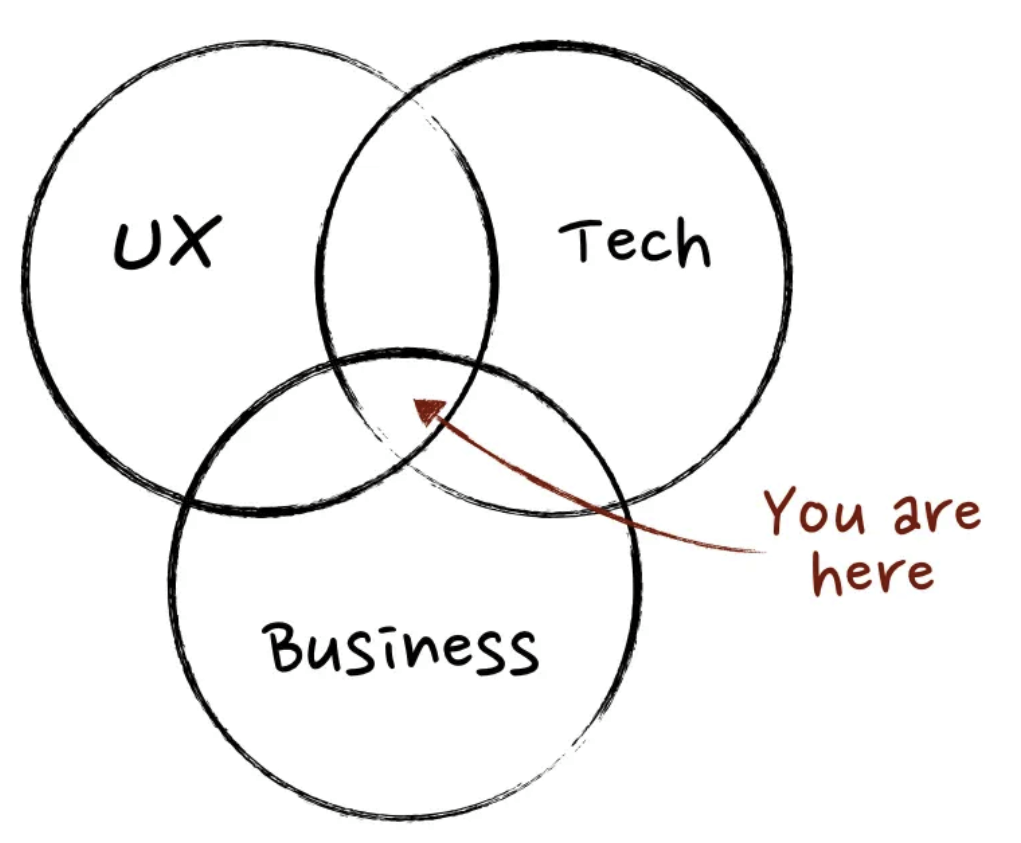
\includegraphics[width=0.5\linewidth]{Degree//static/SE_PM_stuff.png}
        \caption{Product Manager}
    \end{figure}
    \item \textbf{Business}: Works closely with marketing teams and sales, Understand business goals, how the product will maximize return on investment
    \item \textbf{Tech}: Should know the technology stack, Understand the level of effort involved, Take important technical decisions.
    \item \textbf{UX}: Passionate about the user, What does the user want
    \item A good product manager must be experienced in at least one, passionate about all three, and conversant with practitioners in all.
    \item \textbf{Designers}: User Experience (UX) roles, Transform requirements to solutions, Talk to users, create prototypes
    \item \textbf{Software Engineers}: Write code with others in the team to implement requirements, Software engineers don’t get to decide what product is made, or what problems the product solves
    \item \textbf{Engineering Managers}: In large organizations, transmitting information between higher and lower parts, Also known as project manager.
    \item PMs are responsible for Organizing and prioritizing work, Coordinating between different teams, Resolving interpersonal conflict between engineers
    \item \textbf{Sales Team}: Sell the product it to users that marketing team has identified. Provide feedback to marketing, product, and design teams regarding the product, which engineers then address.
    \item \textbf{Support Team}: Resolve problems that clients have, Provide feedback to product, design, and engineering about the product and it’s defects/shortcomings
    \item \textbf{Data Scientists}: Analyze data generated from different teams, users, Help organization make better decisions
    \item \textbf{Ethics and Policy Specialists}: People with background in law, social science, policy, Shape the terms of service of the software product, software licenses, privacy policy etc. Important for any company that works with data
\end{itemize}

\subsection{Communication, Collaboration and Productivity}
\begin{itemize}
    \item \textbf{Conceptual Integration}: Everyone on a team has the same understanding of what is being built and why, Effective communication ensures conceptual integrity
    \item \textbf{Knowledge Sharing Tools}: used for sharing documents and archiving decisions
    \item \textbf{Issue Tracker}: JIRA, Pivotal Tracker, Track different issues, History of who all worked on these issues
    \item \textbf{GitHub Pages}: Many libraries, frameworks are hosted on GitHub
    \item \textbf{Stack Overflow}: Helps to resolve issues that you are facing, Provides links to additional learning resources
    \item Knowledge of one project might be needed in another project. Useful if it is documented and archived properly
    \item When people leave the organization, specialized knowledge goes along with them
    \item Mitigation: “cross-training”, rotating developers between projects
    \item \textbf{Productivity}: Traditionally work done per unit time, this is difficult to define in software engineering, Not necessarily no of lines of code
    \item \textbf{Project Management Tools}: Enables all members of the team to get a big picture as well as detailed view of progress
    \item \textbf{Development Tools}: IDEs, features in IDEs help developers become more productive
\end{itemize}

\subsection{What Makes a Great Software Engineer?}
\begin{itemize}
    \item \textbf{Macro Designs}: design and architecture level, e.g. which libraries, frameworks to use
    \item \textbf{Micro Designs}: Algorithms, data structures for a particular module
    \item Rational Decision-Making Process
    \begin{enumerate}
        \item Identify the decision to be made
        \item Systematically identify alternatives
        \item Think through potential outcomes
        \item Evaluate which of the outcome is best for the given context
        \item Make a decision
    \end{enumerate}
\end{itemize}
\end{document}
